\documentclass[aspectratio=169, 10pt]{beamer}

% ==============================================================================
% THEME & PACKAGES SETUP
% ==============================================================================
\usetheme{Madrid}
\usefonttheme{professionalfonts}

\usepackage[utf8]{inputenc}
\usepackage{amsmath, amssymb, amsfonts}
\usepackage{graphicx}
\usepackage{booktabs}
\usepackage{tikz}
\usetikzlibrary{shapes.geometric, arrows.meta, positioning, calc, backgrounds, fit, decorations.pathreplacing, shadows}
\usepackage{xcolor}
\usepackage{colortbl}
\usepackage{hyperref}
\usepackage{microtype}

% Graphicspath to locate generated result figures seamlessly
\graphicspath{{../results/}{results/}{./}}

% Safe image inclusion macro (renders clean placeholder if file is missing)
\newcommand{\safeincludegraphics}[2][]{%
    \IfFileExists{#2}{%
        \includegraphics[#1]{#2}%
    }{%
        \begin{tikzpicture}
            \node[draw=slate!30, fill=slate!5, dashed, rounded corners=6pt, inner sep=8pt, text width=0.78\linewidth, minimum height=3.8cm, align=center] {
                \textcolor{navy}{\textbf{\small Figure unavailable}}\\[-1pt]
                \textcolor{slate}{\scriptsize\nolinkurl{#2}}\\[4pt]
                \textcolor{slate}{\footnotesize Generate with: \texttt{python notebooks/make\_figures.py}}\\
                \textcolor{slate!70}{\scriptsize (Auto-embeds when present in \texttt{results/})}
            };
        \end{tikzpicture}%
    }%
}

% ==============================================================================
% COLOR PALETTE (Clean, High-Contrast Precision Theme)
% ==============================================================================
\definecolor{navy}{HTML}{0F172A}        % Deep Midnight Navy (Primary)
\definecolor{blueaccent}{HTML}{0284C7}  % Sky Blue (Primary Accent)
\definecolor{teal}{HTML}{0D9488}        % Teal / Aqua
\definecolor{slate}{HTML}{475569}       % Muted Slate Gray
\definecolor{lightbg}{HTML}{F8FAFC}     % Crisp Clean White/Off-White Background
\definecolor{cardbg}{HTML}{FFFFFF}      % Pure White for Cards
\definecolor{cardborder}{HTML}{E2E8F0}  % Light Slate Border
\definecolor{coral}{HTML}{EA580C}       % Coral / Orange
\definecolor{emerald}{HTML}{16A34A}     % Emerald Green
\definecolor{crimson}{HTML}{DC2626}     % Red (Noise / Warning)

% Apply Beamer Colors
\setbeamercolor{palette primary}{bg=navy, fg=white}
\setbeamercolor{palette secondary}{bg=blueaccent, fg=white}
\setbeamercolor{palette tertiary}{bg=slate, fg=white}
\setbeamercolor{palette quaternary}{bg=navy, fg=white}

\setbeamercolor{structure}{fg=blueaccent}
\setbeamercolor{background canvas}{bg=lightbg}
\setbeamercolor{normal text}{fg=navy, bg=lightbg}
\setbeamercolor{frametitle}{bg=navy, fg=white}
\setbeamercolor{title}{bg=navy, fg=white}

% Remove default navigation symbols for a clean, modern look
\setbeamertemplate{navigation symbols}{}

% Custom Headline & Footline
\setbeamertemplate{headline}{}
\setbeamertemplate{footline}{
    \leavevmode%
    \hbox{%
        \begin{beamercolorbox}[wd=.333333\paperwidth,ht=2.4ex,dp=1.0ex,left,leftskip=1.5em]{palette primary}%
            \scriptsize \textbf{Team SevenEight} $\vert$ CSE 220
        \end{beamercolorbox}%
        \begin{beamercolorbox}[wd=.333333\paperwidth,ht=2.4ex,dp=1.0ex,center]{palette primary}%
            \scriptsize Sonar Distance Simulator
        \end{beamercolorbox}%
        \begin{beamercolorbox}[wd=.333333\paperwidth,ht=2.4ex,dp=1.0ex,right,rightskip=1.5em]{palette primary}%
            \scriptsize Slide \insertframenumber{} of \inserttotalframenumber
        \end{beamercolorbox}%
    }%
    \vskip0pt%
}

% Custom Frame Title Styling
\setbeamertemplate{frametitle}{
    \nointerlineskip
    \begin{beamercolorbox}[wd=\paperwidth,ht=3.2ex,dp=1.2ex,leftskip=1.2em]{frametitle}
        \textbf{\small \insertframetitle}
        \ifx\insertframesubtitle\@empty\else
            ~~\textcolor{blueaccent}{\scriptsize$\vert$~~}\textcolor{blueaccent!30}{\tiny \insertframesubtitle}
        \fi
    \end{beamercolorbox}
}

% ==============================================================================
% METADATA
% ==============================================================================
\title[\textbf{Sonar Distance Simulator}]{\textbf{\LARGE Sonar Distance Simulator}}
\subtitle{\large Pulse-Echo Ranging, Matched Filtering, and Resolution Analysis}
\author[\textbf{Team SevenEight}]{%
    \textbf{Aditya Tirtho Roy} (2305178) \and \textbf{Farhan Ehsas Sami} (2305177)%
}
\institute[BUET CSE]{%
    Department of Computer Science and Engineering, BUET\\[2pt]
    \textcolor{blueaccent}{\textbf{CSE 220: Signals and Systems Laboratory}}
}
\date{Final Project Evaluation}

% ==============================================================================
% DOCUMENT BODY
% ==============================================================================
\begin{document}

% ------------------------------------------------------------------------------
% SLIDE 1: TITLE SLIDE
% ------------------------------------------------------------------------------
\begin{frame}[plain]
    \begin{tikzpicture}[remember picture, overlay]
        \fill[navy] (current page.south west) rectangle (current page.north east);
        \fill[blueaccent!15, opacity=0.08] (current page.north east) circle (6.5cm);
        \fill[teal!20, opacity=0.05] (current page.south west) circle (5cm);
    \end{tikzpicture}
    
    \vspace{0.3cm}
    \begin{center}
        \textcolor{blueaccent}{\textbf{\scriptsize CSE 220 SIGNALS AND SYSTEMS $\cdot$ FINAL EVALUATION}}\\[6pt]
        {\textcolor{white}{\textbf{\Huge Sonar Distance Simulator}}}\\[6pt]
        {\textcolor{blueaccent!90}{\large \textit{Pulse-Echo Ranging, Matched Filtering, and Range Resolution Limits}}}\\[16pt]
        
        
\begin{tikzpicture}
            \node[fill=white, fill opacity=0.10, text opacity=1, draw=white, draw opacity=0.30, rounded corners=6pt, inner sep=9pt, text width=0.84\linewidth, align=center] {
                \textcolor{white}{\textbf{\normalsize Team SevenEight}}\\[5pt]
                \textcolor{white}{\textbf{Aditya Tirtho Roy}} \textcolor{blueaccent!60}{(2305178)} \quad$\vert$\quad
                \textcolor{white}{\textbf{Farhan Ehsas Sami}} \textcolor{blueaccent!60}{(2305177)}\\[3pt]
                \textcolor{slate!30}{\footnotesize Department of Computer Science and Engineering, BUET}
            };
        \end{tikzpicture}
        
        \vspace{10pt}
        \textcolor{slate!30}{\scriptsize Pure DSP Core $\cdot$ Monte Carlo Analysis $\cdot$ Streamlit Instrument UI $\cdot$ Real Hardware Ranging}
    \end{center}
\end{frame}

% ------------------------------------------------------------------------------
% SLIDE 2: THE PROBLEM (VISUAL & MINIMALIST)
% ------------------------------------------------------------------------------
\begin{frame}{The Problem: Finding Buried Echoes in Noise}{Pulse-Echo Ranging in Theory vs. Physical Reality}
    \centering
    
    % Visual Physics Diagram
    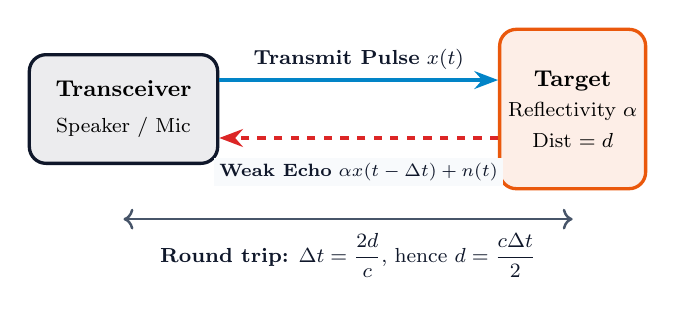
\begin{tikzpicture}[scale=0.92, transform shape]
        % Transceiver
        \node[draw=navy, fill=navy!8, rounded corners=6pt, line width=1.2pt, minimum width=2.6cm, minimum height=1.5cm, align=center] (tx) at (0, 1.8) {
            \textbf{\small Transceiver}\\[2pt]
            \footnotesize Speaker / Mic
        };
        
        % Target
        \node[draw=coral, fill=coral!10, rounded corners=6pt, line width=1.2pt, minimum width=1.6cm, minimum height=2.2cm, align=center] (target) at (6.2, 1.8) {
            \textbf{\small Target}\\
            \footnotesize Reflectivity $\alpha$\\
            \footnotesize Dist $= d$
        };
        
        % Outgoing Wave
        \draw[-{Stealth[length=3mm]}, blueaccent, line width=1.6pt] ($(tx.east)+(0,0.4)$) -- node[above, text=navy, font=\footnotesize] {\textbf{Transmit Pulse} $x(t)$} ($(target.west)+(0,0.4)$);
        
        % Reflected Wave
        \draw[-{Stealth[length=3mm]}, crimson, line width=1.6pt, dashed] ($(target.west)+(0,-0.4)$) -- node[below=7pt, text=navy, font=\scriptsize, fill=lightbg, inner sep=2pt] {\textbf{Weak Echo} $\alpha x(t-\Delta t)+n(t)$} ($(tx.east)+(0,-0.4)$);
        
        % Round-trip indicator
        \draw[<->, slate, line width=0.9pt] (0, 0.28) -- node[below=2pt, font=\footnotesize, text=navy] {\textbf{Round trip:} $\Delta t = \dfrac{2d}{c}$, hence $d = \dfrac{c\Delta t}{2}$} (6.2, 0.28);
    \end{tikzpicture}
    
    \vspace{8pt}
    
    % Three Minimal Callout Cards
    \begin{columns}[T]
        \begin{column}{0.32\textwidth}
            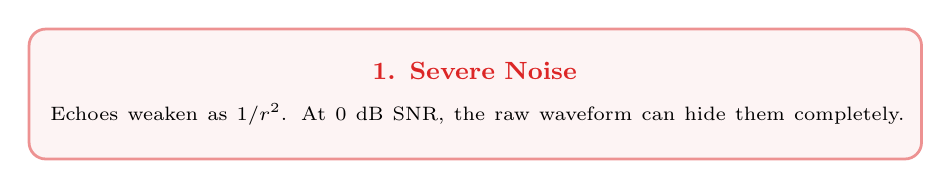
\begin{tikzpicture}
                \node[draw=crimson!50, fill=crimson!5, rounded corners=6pt, line width=1pt, text width=0.90\linewidth, minimum height=1.65cm, inner sep=6pt, align=center] {
                    \textcolor{crimson}{\textbf{\small 1. Severe Noise}}\\[3pt]
                    \scriptsize Echoes weaken as $1/r^2$.
                    At $0\text{ dB}$ SNR, the raw
                    waveform can hide them completely.
                };
            \end{tikzpicture}
        \end{column}
        \begin{column}{0.32\textwidth}
            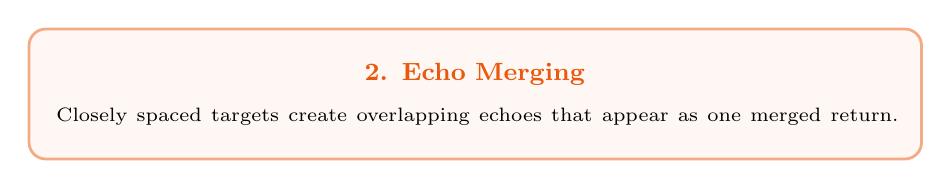
\begin{tikzpicture}
                \node[draw=coral!50, fill=coral!5, rounded corners=6pt, line width=1pt, text width=0.90\linewidth, minimum height=1.65cm, inner sep=6pt, align=center] {
                    \textcolor{coral}{\textbf{\small 2. Echo Merging}}\\[3pt]
                    \scriptsize Closely spaced targets create
                    overlapping echoes that appear
                    as one merged return.
                };
            \end{tikzpicture}
        \end{column}
        \begin{column}{0.32\textwidth}
            
\begin{tikzpicture}
                \node[draw=blueaccent!50, fill=blueaccent!5, rounded corners=6pt, line width=1pt, text width=0.90\linewidth, minimum height=1.65cm, inner sep=6pt, align=center] {
                    \textcolor{blueaccent}{\textbf{\small 3. Energy Dilemma}}\\[3pt]
                    \scriptsize Short pulses resolve targets
                    but carry little energy; long pulses
                    are stronger but blur targets.
                };
            \end{tikzpicture}
        \end{column}
    \end{columns}
\end{frame}

% ------------------------------------------------------------------------------
% SLIDE 3: INTUITIVE INPUT-OUTPUT MODEL (KEY REQUIREMENT)
% ------------------------------------------------------------------------------
\begin{frame}{Intuitive System Model: Input vs. Output}{A Complete Black-Box View of the Sonar Simulator}
    \centering
    
    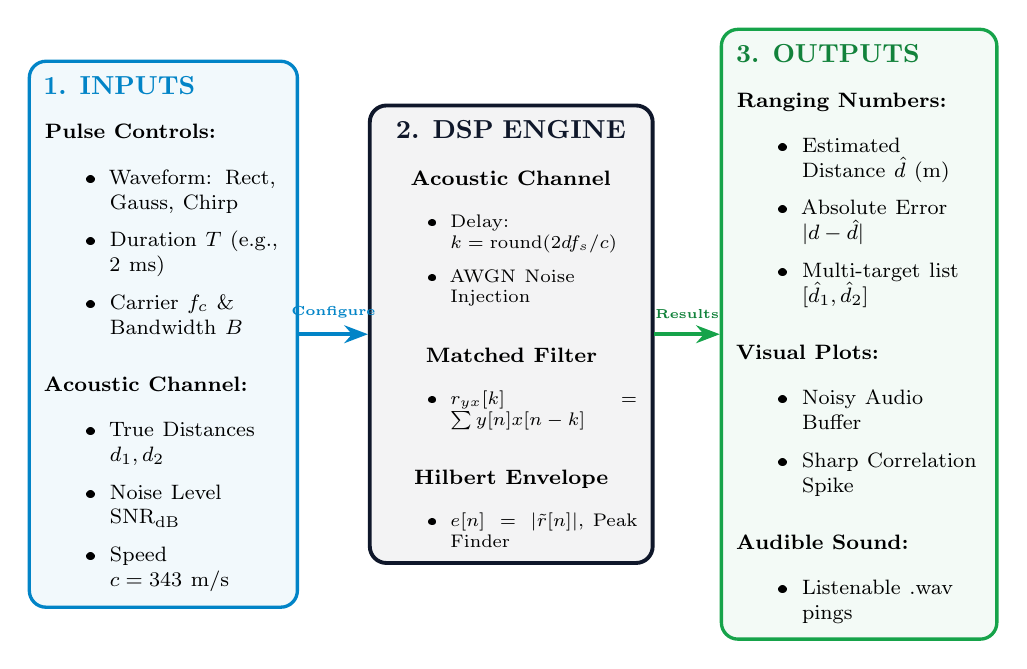
\begin{tikzpicture}[scale=0.94, transform shape,
        node distance=0.8cm and 0.8cm,
        box/.style={draw=navy, fill=white, rounded corners=6pt, line width=1.1pt, inner sep=6pt},
        inbox/.style={draw=blueaccent, fill=blueaccent!5, rounded corners=6pt, line width=1.2pt, text width=3.2cm, minimum height=5.1cm, inner sep=6pt},
        proc/.style={draw=navy, fill=navy!5, rounded corners=6pt, line width=1.4pt, text width=3.4cm, minimum height=5.1cm, inner sep=6pt, align=center},
        outbox/.style={draw=emerald, fill=emerald!5, rounded corners=6pt, line width=1.2pt, text width=3.3cm, minimum height=5.1cm, inner sep=6pt},
        arr/.style={-{Stealth[length=3mm]}, line width=1.6pt}
    ]
        % INPUTS
        \node[inbox] (inp) at (-4.7, 0) {
            \textcolor{blueaccent}{\textbf{\normalsize 1. INPUTS}}\\[5pt]
            \textbf{\footnotesize Pulse Controls:}
            \begin{itemize}\footnotesize\setlength\itemsep{1pt}
                \item Waveform: Rect, Gauss, Chirp
                \item Duration $T$ (e.g., $2\text{ ms}$)
                \item Carrier $f_c$ \& Bandwidth $B$
            \end{itemize}
            \vspace{2pt}
            \textbf{\footnotesize Acoustic Channel:}
            \begin{itemize}\footnotesize\setlength\itemsep{1pt}
                \item True Distances $d_1, d_2$
                \item Noise Level $\text{SNR}_{\text{dB}}$
                \item Speed $c = 343\text{ m/s}$
            \end{itemize}
        };

        % PROCESSING ENGINE
        \node[proc] (engine) at (0, 0) {
            \textcolor{navy}{\textbf{\normalsize 2. DSP ENGINE}}\\[6pt]
            \textbf{\footnotesize Acoustic Channel}
            \begin{itemize}\scriptsize\setlength\itemsep{1pt}
                \item Delay: $k = \text{round}(2d f_s / c)$
                \item AWGN Noise Injection
            \end{itemize}
            \vspace{3pt}
            \textbf{\footnotesize Matched Filter}
            \begin{itemize}\scriptsize\setlength\itemsep{1pt}
                \item $r_{yx}[k] = \sum y[n] x[n-k]$
            \end{itemize}
            \vspace{3pt}
            \textbf{\footnotesize Hilbert Envelope}
            \begin{itemize}\scriptsize\setlength\itemsep{1pt}
                \item $e[n] = |\tilde{r}[n]|$, Peak Finder
            \end{itemize}
        };

        % OUTPUTS
        \node[outbox] (out) at (4.7, 0) {
            \textcolor{emerald!80!black}{\textbf{\normalsize 3. OUTPUTS}}\\[5pt]
            \textbf{\footnotesize Ranging Numbers:}
            \begin{itemize}\footnotesize\setlength\itemsep{1pt}
                \item Estimated Distance $\hat{d}$ (m)
                \item Absolute Error $|d - \hat{d}|$
                \item Multi-target list $[\hat{d}_1, \hat{d}_2]$
            \end{itemize}
            \vspace{2pt}
            \textbf{\footnotesize Visual Plots:}
            \begin{itemize}\footnotesize\setlength\itemsep{1pt}
                \item Noisy Audio Buffer
                \item Sharp Correlation Spike
            \end{itemize}
            \vspace{2pt}
            \textbf{\footnotesize Audible Sound:}
            \begin{itemize}\footnotesize\setlength\itemsep{1pt}
                \item Listenable .wav pings
            \end{itemize}
        };

        % CONNECTORS
        \draw[arr, blueaccent] (inp.east) -- node[midway, above=2pt, font=\tiny\bfseries, text=blueaccent] {Configure} (engine.west);
        \draw[arr, emerald] (engine.east) -- node[midway, above=2pt, font=\tiny\bfseries, text=emerald!80!black] {Results} (out.west);
    \end{tikzpicture}
    
    \vspace{2pt}
    
\begin{tikzpicture}
        \node[draw=slate!30, fill=white, rounded corners=4pt, inner sep=4pt, text width=0.92\linewidth, align=center] {
            \scriptsize \textbf{Core Takeaway:} Configure the pulse and scene, then receive distance estimates, diagnostic plots, and audible sonar clips.
        };
    \end{tikzpicture}
\end{frame}

% ------------------------------------------------------------------------------
% SLIDE 4: MATCHED FILTERING (GRAPHICAL EXPLANATION)
% ------------------------------------------------------------------------------
\begin{frame}{Core Theory: Matched Filtering}{How Cross-Correlation Extracts Buried Signals from Noise}
    \begin{columns}[T]
        \begin{column}{0.48\textwidth}
            \textbf{\textcolor{navy}{Sliding Template Cross-Correlation:}}
            \begin{itemize}\small
                \item Mathematically optimal filter in AWGN (Cauchy-Schwarz Inequality):
                $$r_{yx}[k] = \sum_{n} y[n] \, x[n-k]$$
                \item \textbf{Intuition:} 
                \begin{itemize}\footnotesize
                    \item Where there is only noise $\to$ multiplies random numbers $\to$ \textbf{averages to zero}.
                    \item Where the echo matches the template $\to$ multiplies in-phase $\to$ \textbf{constructive surge}!
                \end{itemize}
                \item \textbf{Peak to Distance:}
                $$\hat{d} = \frac{(k_{\text{peak}} - \text{offset}) \cdot c}{2 f_s}$$
            \end{itemize}
        \end{column}
        
        \begin{column}{0.50\textwidth}
            % Intuitive Sliding Graphic
            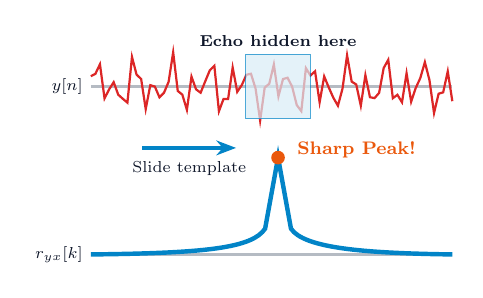
\begin{tikzpicture}[scale=0.82, transform shape]
                % 1. Noisy Buffer
                \draw[slate!40, line width=0.8pt] (0, 3.4) -- (5.6, 3.4);
                \draw[crimson, line width=0.8pt] plot[domain=0:5.6, samples=80] (\x, {3.4 + 0.22*sin(1200*\x) + 0.16*cos(2800*\x) + 0.18*sin(650*\x)});
                \node[left, font=\scriptsize, text=navy] at (0, 3.4) {$y[n]$};
                \draw[blueaccent, fill=blueaccent!15, opacity=0.7] (2.4, 2.9) rectangle (3.4, 3.9);
                \node[above, font=\scriptsize, text=navy] at (2.9, 3.9) {\textbf{Echo hidden here}};
                
                % 2. Sliding Pulse
                \draw[-{Stealth[length=2.5mm]}, blueaccent, line width=1.4pt] (0.8, 2.45) -- (2.25, 2.45)
                    node[midway, below=2pt, font=\scriptsize, text=navy] {Slide template};
                
                % 3. Correlation Spike
                \draw[slate!40, line width=0.8pt] (0, 0.8) -- (5.6, 0.8);
                \draw[blueaccent, line width=1.6pt] (0, 0.8) .. controls (1.8, 0.82) and (2.5, 0.9) .. (2.7, 1.2) -- (2.9, 2.3) -- (3.1, 1.2) .. controls (3.3, 0.9) and (4.2, 0.82) .. (5.6, 0.8);
                \node[left, font=\scriptsize, text=navy] at (0, 0.8) {$r_{yx}[k]$};
                \fill[coral] (2.9, 2.3) circle (3pt);
                \node[above right=1pt, font=\footnotesize, text=coral] at (3.05,2.15) {\textbf{Sharp Peak!}};
            \end{tikzpicture}
            
            \vspace{6pt}
            
\begin{tikzpicture}
                \node[draw=emerald!50, fill=emerald!5, rounded corners=4pt, inner sep=4pt, text width=0.94\linewidth, align=center] {
                    \footnotesize \textbf{The Aha! Moment:} Even when noise is louder than the echo ($0\text{ dB}$ SNR), the matched filter recovers the echo with sub-millimeter precision!
                };
            \end{tikzpicture}
        \end{column}
    \end{columns}
\end{frame}

% ------------------------------------------------------------------------------
% SLIDE 5: MULTI-TARGET & THE HILBERT ENVELOPE (GRAPHICAL)
% ------------------------------------------------------------------------------
\begin{frame}{Multiple Targets: The Hilbert Analytic Envelope}{Overcoming Carrier Ripple to Accurately Count Echoes}
    \begin{columns}[T]
        \begin{column}{0.48\textwidth}
            \textbf{\textcolor{crimson}{1. The Carrier Trap (Raw Correlation):}}
            \begin{itemize}\small
                \item Carrier oscillates at $4\text{ kHz}$.
                \item Raw correlation produces \textbf{15--20 cycle ripples} for just 2 true targets!
                \item Simple thresholding counts false targets.
            \end{itemize}
            
            \vspace{6pt}
            \textbf{\textcolor{emerald!80!black}{2. The Solution (Hilbert Envelope):}}
            \begin{itemize}\small
                \item Construct analytic signal:
                $$\tilde{r}[n] = r[n] + j \mathcal{H}\{r[n]\}$$
                \item Smooth envelope: $e[n] = |\tilde{r}[n]|$.
                \item Peak finder on $e[n]$ detects \textbf{exactly 2 true target crests}!
            \end{itemize}
        \end{column}
        
        \begin{column}{0.50\textwidth}
            % Hilbert Envelope Graphical Comparison
            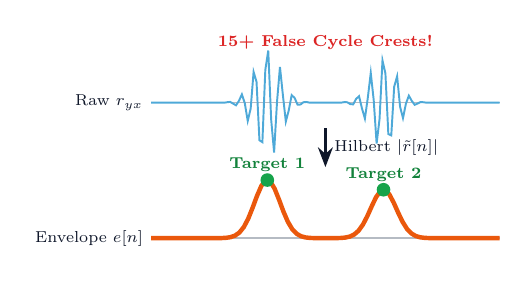
\begin{tikzpicture}[scale=0.82, transform shape]
                % Raw Oscillation
                \draw[slate!40, line width=0.6pt] (0, 2.5) -- (5.4, 2.5);
                \draw[blueaccent!70, line width=0.7pt] plot[domain=0:5.4, samples=120] (\x, {2.5 + (0.9*exp(-(\x-1.8)^2/0.08) + 0.75*exp(-(\x-3.6)^2/0.08))*cos(1800*\x)});
                \node[left, font=\scriptsize, text=navy] at (0, 2.5) {Raw $r_{yx}$};
                \node[above, font=\scriptsize, text=crimson] at (2.7, 3.2) {\textbf{15+ False Cycle Crests!}};
                
                % Arrow
                \draw[-{Stealth[length=2.5mm]}, navy, line width=1.3pt] (2.7, 2.1) -- (2.7, 1.5) node[midway, right, font=\scriptsize] {Hilbert $|\tilde{r}[n]|$};
                
                % Smooth Envelope
                \draw[slate!40, line width=0.6pt] (0, 0.4) -- (5.4, 0.4);
                \draw[coral, line width=1.6pt] plot[domain=0:5.4, samples=80] (\x, {0.4 + 0.9*exp(-(\x-1.8)^2/0.08) + 0.75*exp(-(\x-3.6)^2/0.08)});
                \node[left, font=\scriptsize, text=navy] at (0, 0.4) {Envelope $e[n]$};
                
                \fill[emerald] (1.8, 1.3) circle (3pt) node[above, font=\scriptsize, text=emerald!80!black] {\textbf{Target 1}};
                \fill[emerald] (3.6, 1.15) circle (3pt) node[above, font=\scriptsize, text=emerald!80!black] {\textbf{Target 2}};
            \end{tikzpicture}
            
            \vspace{4pt}
            
\begin{tikzpicture}
                \node[draw=slate!30, fill=white, rounded corners=4pt, inner sep=4pt, text width=0.94\linewidth, align=center] {
                    \footnotesize \textbf{Rule of Thumb:} Raw $\text{argmax}$ for single targets (sharpest); Hilbert envelope for multi-targets (eliminates carrier cycle ripples).
                };
            \end{tikzpicture}
        \end{column}
    \end{columns}
\end{frame}

% ------------------------------------------------------------------------------
% SLIDE 6: RANGE RESOLUTION & CHIRP (GRAPHICAL)
% ------------------------------------------------------------------------------
\begin{frame}{Range Resolution: Why We Need Chirps}{Breaking the Classical Pulse-Length / Energy Trade-off}
    \begin{columns}[T]
        \begin{column}{0.48\textwidth}
            \textbf{\textcolor{navy}{The Rayleigh Resolution Limit:}}
            $$\Delta R_{\text{min}} \approx \frac{c}{2B}$$
            Two targets can only be separated if their echo gap exceeds the pulse's correlation width.
            
            \vspace{6pt}
            \textbf{\textcolor{crimson}{The Classical Trade-Off (Tone Bursts):}}
            \begin{itemize}\small
                \item Bandwidth is tied to duration: $B \approx 1/T$.
                \item To separate close targets $\to$ must make pulse tiny $\to$ carries tiny energy $\to$ ruined by noise!
            \end{itemize}
            
            \vspace{4pt}
            \textbf{\textcolor{emerald!80!black}{The Chirp (LFM) Breakthrough:}}
            \begin{itemize}\small
                \item Sweeps frequency over time ($f_0 \to f_0 + B$).
                \item \textbf{Decouples duration $T$ from bandwidth $B$}: high energy + razor-sharp resolution!
            \end{itemize}
        \end{column}
        
        \begin{column}{0.50\textwidth}
            % Chirp Pulse Compression Graphic
            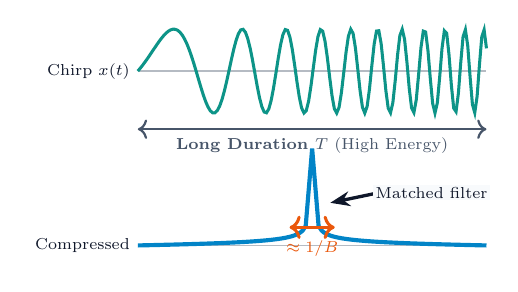
\begin{tikzpicture}[scale=0.82, transform shape]
                % Chirp
                \draw[slate!40, line width=0.6pt] (0, 2.7) -- (5.4, 2.7);
                \draw[teal, line width=1.1pt] plot[domain=0:5.4, samples=150] (\x, {2.7 + 0.65*sin((100 + 110*\x)*\x)});
                \node[left, font=\scriptsize, text=navy] at (0, 2.7) {Chirp $x(t)$};
                \draw[<->, slate, line width=0.8pt] (0, 1.8) -- node[below, font=\scriptsize] {\textbf{Long Duration $T$} (High Energy)} (5.4, 1.8);
                
                % Compression arrow, offset from the peak for visual clarity
                \draw[-{Stealth[length=2.5mm]}, navy, line width=1.2pt] (3.75, 0.82) -- (2.98, 0.66);
                \node[fill=lightbg, inner sep=1pt, font=\scriptsize, text=navy] at (4.55,0.82) {Matched filter};
                
                % Compressed Spike
                \draw[slate!40, line width=0.6pt] (0, 0) -- (5.4, 0);
                \draw[blueaccent, line width=1.5pt] (0, 0) .. controls (2.3, 0.05) and (2.5, 0.1) .. (2.6, 0.3) -- (2.7, 1.5) -- (2.8, 0.3) .. controls (2.9, 0.1) and (3.1, 0.05) .. (5.4, 0);
                \node[left, font=\scriptsize, text=navy] at (0, 0) {Compressed};
                \draw[<->, coral, line width=1.1pt] (2.35, 0.28) -- node[below=2pt, font=\scriptsize, text=coral] {$\approx 1/B$} (3.05, 0.28);
            \end{tikzpicture}
            
            \vspace{4pt}
            
\begin{tikzpicture}
                \node[draw=teal!50, fill=teal!5, rounded corners=4pt, inner sep=4pt, text width=0.94\linewidth, align=center] {
                    \footnotesize \textbf{Pulse Compression:} Long duration plus wide bandwidth gives high energy and a narrow $\approx 1/B$ correlation peak.
                };
            \end{tikzpicture}
        \end{column}
    \end{columns}
\end{frame}

% ------------------------------------------------------------------------------
% SLIDE 7: SOFTWARE ARCHITECTURE (CLEAN DIAGRAM)
% ------------------------------------------------------------------------------
\begin{frame}{Software Architecture \& Engineering Discipline}{A Clean, Reusable Pure-DSP Core with Zero UI Side Effects}
    \begin{columns}[T]
        \begin{column}{0.45\textwidth}
            \begin{block}{\textbf{The Golden Rule}}
                \textit{Functions in \texttt{src/} take numbers/arrays and return numbers/arrays. They NEVER call \texttt{plt.show()} or \texttt{print()}.}
            \end{block}
            
            \vspace{6pt}
            \textbf{\textcolor{navy}{Why This Matters:}}
            \begin{itemize}\small
                \item \textbf{100\% Reusable DSP Core:} Tests, report figures, and the Streamlit web app call the \textbf{exact same functions}.
                \item \textbf{Zero UI Coupling:} Front-end UI redesigns never risk breaking core physics calculations.
                \item \textbf{Fully Automated:} 33 passing pytest tests + 17 pulse physics verification checks.
            \end{itemize}
        \end{column}
        
        \begin{column}{0.53\textwidth}
            % Modular Architecture Diagram
            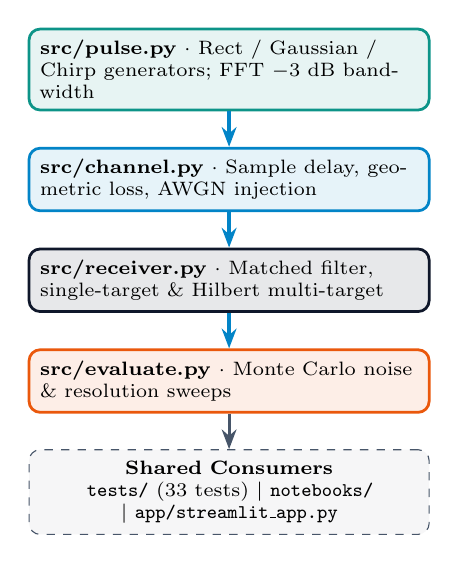
\begin{tikzpicture}[
                node distance=0.45cm,
                layer/.style={draw=navy, fill=white, rounded corners=4pt, line width=1pt, text width=4.8cm, inner sep=4pt, font=\scriptsize},
                arr/.style={-{Stealth[length=2.5mm]}, line width=1.2pt, draw=blueaccent}
            ]
                \node[layer, fill=teal!10, draw=teal] (pulse) {
                    \textbf{src/pulse.py} $\cdot$ Rect / Gaussian / Chirp generators; FFT $-3\text{ dB}$ bandwidth
                };
                \node[layer, fill=blueaccent!10, draw=blueaccent, below=of pulse] (chan) {
                    \textbf{src/channel.py} $\cdot$ Sample delay, geometric loss, AWGN injection
                };
                \node[layer, fill=navy!10, draw=navy, below=of chan] (rx) {
                    \textbf{src/receiver.py} $\cdot$ Matched filter, single-target \& Hilbert multi-target
                };
                \node[layer, fill=coral!10, draw=coral, below=of rx] (eval) {
                    \textbf{src/evaluate.py} $\cdot$ Monte Carlo noise \& resolution sweeps
                };
                
                \draw[arr] (pulse) -- (chan);
                \draw[arr] (chan) -- (rx);
                \draw[arr] (rx) -- (eval);
                
                \node[draw=slate, dashed, rounded corners=4pt, fill=slate!5, text width=4.8cm, inner sep=4pt, below=0.45cm of eval, font=\scriptsize, align=center] (consumers) {
                    \textbf{Shared Consumers}\\
                    \texttt{tests/} (33 tests) $\vert$ \texttt{notebooks/} $\vert$ \texttt{app/streamlit\_app.py}
                };
                \draw[-{Stealth[length=2.5mm]}, slate, line width=1.1pt] (eval) -- (consumers);
            \end{tikzpicture}
        \end{column}
    \end{columns}
\end{frame}

% ------------------------------------------------------------------------------
% SLIDE 8: END-TO-END PIPELINE IN ACTION (FIG 2)
% ------------------------------------------------------------------------------
\begin{frame}{Experimental Results: Pipeline in Action}{Recovering a Target Buried in Severe Noise ($0\text{ dB}$ SNR)}
    \begin{columns}[T]
        \begin{column}{0.68\textwidth}
            \centering
            \safeincludegraphics[width=0.98\linewidth]{fig2_pipeline.png}
        \end{column}
        
        \begin{column}{0.30\textwidth}
            \vspace{4pt}
            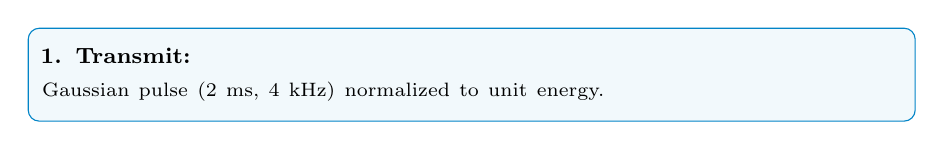
\begin{tikzpicture}
                \node[draw=blueaccent, fill=blueaccent!5, rounded corners=4pt, text width=0.90\linewidth, minimum height=1.18cm, inner sep=5pt] {
                    \textbf{\footnotesize 1. Transmit:}\\
                    \scriptsize Gaussian pulse ($2\text{ ms}$, $4\text{ kHz}$) normalized to unit energy.
                };
            \end{tikzpicture}
            
            \vspace{4pt}
            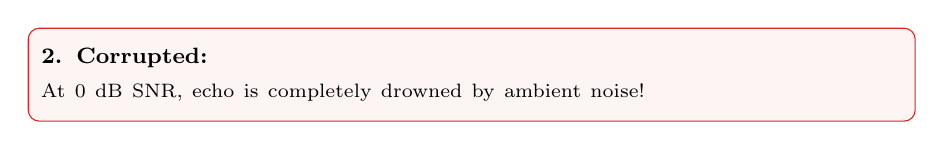
\begin{tikzpicture}
                \node[draw=crimson, fill=crimson!5, rounded corners=4pt, text width=0.90\linewidth, minimum height=1.18cm, inner sep=5pt] {
                    \textbf{\footnotesize 2. Corrupted:}\\
                    \scriptsize At $0\text{ dB}$ SNR, echo is completely drowned by ambient noise!
                };
            \end{tikzpicture}
            
            \vspace{4pt}
            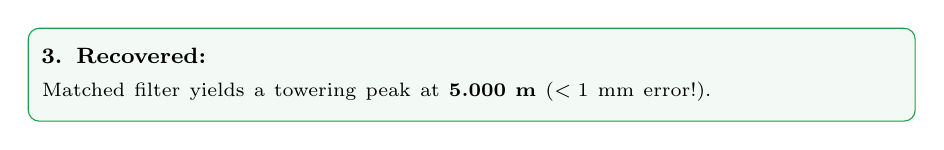
\begin{tikzpicture}
                \node[draw=emerald, fill=emerald!5, rounded corners=4pt, text width=0.90\linewidth, minimum height=1.18cm, inner sep=5pt] {
                    \textbf{\footnotesize 3. Recovered:}\\
                    \scriptsize Matched filter yields a towering peak at \textbf{5.000 m} ($<1\text{ mm}$ error!).
                };
            \end{tikzpicture}
        \end{column}
    \end{columns}
\end{frame}

% ------------------------------------------------------------------------------
% SLIDE 9: TRANSMIT PULSES & BANDWIDTH (FIG 1)
% ------------------------------------------------------------------------------
\begin{frame}{Experimental Results: Pulse Types \& Spectra}{Understanding Transmit Waveforms in Time and Frequency}
    \begin{columns}[T]
        \begin{column}{0.68\textwidth}
            \centering
            \safeincludegraphics[width=0.98\linewidth]{fig1_pulse_types.png}
        \end{column}
        
        \begin{column}{0.30\textwidth}
            \vspace{6pt}
            \textbf{\textcolor{navy}{\small Waveform Comparison:}}
            \begin{itemize}\footnotesize\setlength\itemsep{4pt}
                \item \textbf{Rect:} Abrupt on/off switch $\to$ heavy spectral splatter.
                \item \textbf{Gaussian:} Bell envelope $\to$ smooth, clean spectrum.
                \item \textbf{Chirp:} Linear frequency sweep $\to$ wide $-3\text{ dB}$ bandwidth for sharp target separation.
            \end{itemize}
            
            \vspace{6pt}
            
\begin{tikzpicture}
                \node[draw=teal!50, fill=teal!5, rounded corners=4pt, inner sep=4pt, text width=0.92\linewidth, align=center] {
                    \scriptsize \textbf{Key Metric:} A wider $-3\text{ dB}$ spectral lobe yields a sharper correlation peak.
                };
            \end{tikzpicture}
        \end{column}
    \end{columns}
\end{frame}

% ------------------------------------------------------------------------------
% SLIDE 10: NOISE RESILIENCE & BREAKDOWN CLIFF (FIG 3)
% ------------------------------------------------------------------------------
\begin{frame}{Experimental Results: Noise Resilience (SNR vs. RMSE)}{Characterizing the System Quantization Floor and Noise Cliff}
    \begin{columns}[T]
        \begin{column}{0.62\textwidth}
            \centering
            \safeincludegraphics[width=0.98\linewidth]{fig3_rmse_vs_snr.png}
        \end{column}
        
        \begin{column}{0.36\textwidth}
            \vspace{2pt}
            \textbf{\textcolor{navy}{\small Key Observations:}}
            
            \vspace{3pt}
            \textbf{\footnotesize 1. Quantization Floor ($\approx 1.8\text{ mm}$):}
            \begin{itemize}\scriptsize
                \item Above $0\text{ dB}$, error is flat.
                \item Arises from discrete sampling:
                $$\text{Floor} \approx \frac{c}{4 f_s} \approx 1.79\text{ mm}$$
            \end{itemize}
            
            \vspace{2pt}
            \textbf{\footnotesize 2. The Threshold Cliff:}
            \begin{itemize}\scriptsize
                \item Below $-4\text{ dB}$, noise spikes eclipse the echo peak, causing rapid breakdown.
            \end{itemize}
            
            \vspace{2pt}
            \textbf{\footnotesize 3. Bandpass Filter Overlap:}
            \begin{itemize}\scriptsize
                \item Pre-filtering coincides with raw matched filter $\to$ confirms matched filter is already optimal for white noise!
            \end{itemize}
        \end{column}
    \end{columns}
\end{frame}

% ------------------------------------------------------------------------------
% SLIDE 11: TWO TARGETS: RESOLVED VS. MERGED (FIG 4 & 5)
% ------------------------------------------------------------------------------
\begin{frame}{Experimental Results: Range Resolution \& Multipath}{Validating the Theoretical Resolution Bound $\Delta R \approx c/(2B)$}
    \begin{columns}[T]
        \begin{column}{0.50\textwidth}
            \centering
            \textbf{\textcolor{navy}{\footnotesize Multipath Separation (40 cm vs. 8 cm)}}
            
            \vspace{2pt}
            \safeincludegraphics[width=0.98\linewidth]{fig5_multipath.png}
            
            \begin{itemize}\scriptsize
                \item \textbf{40 cm gap:} Two distinct peaks resolved.
                \item \textbf{8 cm gap:} Echoes merge into a single wide blob.
            \end{itemize}
        \end{column}
        
        \begin{column}{0.50\textwidth}
            \centering
            \textbf{\textcolor{navy}{\footnotesize Measured Resolution vs. Bandwidth}}
            
            \vspace{2pt}
            \safeincludegraphics[width=0.98\linewidth]{fig4_resolution_vs_bandwidth.png}
            
            \begin{itemize}\scriptsize
                \item Measured points track theoretical dashed curve $c/(2B)$ across a $23\times$ bandwidth range.
                \item Chirps fix duration at $2\text{ ms}$ while sweeping bandwidth.
            \end{itemize}
        \end{column}
    \end{columns}
\end{frame}

% ------------------------------------------------------------------------------
% SLIDE 12: REAL ACOUSTIC HARDWARE VALIDATION (FIG 6)
% ------------------------------------------------------------------------------
\begin{frame}{Physical Validation: Real Laptop Speaker \& Mic Ranging}{Testing the DSP Pipeline in Physical Room Acoustics}
    \begin{columns}[T]
        \begin{column}{0.50\textwidth}
            \textbf{\textcolor{navy}{\small 4-Step Hardware Acoustic Pipeline:}}
            \begin{enumerate}\footnotesize\setlength\itemsep{2pt}
                \item \textbf{Windowed Chirp:} $2\text{--}8\text{ kHz}$ sweep shaped to laptop speaker response.
                \item \textbf{Direct-Path Sync:} Lock onto speaker-to-mic direct bleed as $t = 0$ origin.
                \item \textbf{Frame Folding:} Coherently average 16 bursts $\to$ cancels room noise.
                \item \textbf{Clutter Removal:} Subtract empty-room baseline $\to$ removes furniture reflections and speaker ring.
            \end{enumerate}
            
            \vspace{4pt}
            \begin{table}\scriptsize
                \centering
                \begin{tabular}{lccc}
                    \toprule
                    \textbf{Target} & \textbf{Truth} & \textbf{Measured} & \textbf{Quality} \\
                    \midrule
                    Room Wall & $\approx 1.80\text{ m}$ & \textbf{1.797 m} & \textbf{6.7} $\sigma$ \\
                    Raised Hand & $\approx 0.30\text{ m}$ & \textbf{0.272 m} & \textbf{6.2} $\sigma$ \\
                    \bottomrule
                \end{tabular}
            \end{table}
        \end{column}
        
        \begin{column}{0.48\textwidth}
            \centering
            \safeincludegraphics[width=0.98\linewidth]{fig6_acoustic.png}
            
            \vspace{2pt}
            
\begin{tikzpicture}
                \node[draw=emerald!50, fill=emerald!5, rounded corners=4pt, inner sep=4pt, text width=0.95\linewidth, align=center] {
                    \scriptsize \textbf{Statistical Confidence:} Both detections exceed $>6.0\sigma$ above background clutter! Bit-for-bit verified in \texttt{tests/test\_acoustic.py}.
                };
            \end{tikzpicture}
        \end{column}
    \end{columns}
\end{frame}

% ------------------------------------------------------------------------------
% SLIDE 13: INTERACTIVE STREAMLIT APPLICATION
% ------------------------------------------------------------------------------
\begin{frame}{Interactive Streamlit Application}{A Virtual Laboratory Instrument for Real-Time Exploration}
    \begin{columns}[T]
        \begin{column}{0.50\textwidth}
            \textbf{\textcolor{navy}{\small Four Dedicated Operating Modes:}}
            
            \vspace{3pt}
            \begin{enumerate}\small\setlength\itemsep{3pt}
                \item \textbf{01: Single Target Ranging}
                \begin{itemize}\scriptsize
                    \item Real-time sliders for distance, SNR, and pulse shape.
                \end{itemize}
                \item \textbf{02: Multi-Target Resolution}
                \begin{itemize}\scriptsize
                    \item Live separation slider and dynamic bandwidth sweep.
                \end{itemize}
                \item \textbf{03: Noise Resilience Benchmark}
                \begin{itemize}\scriptsize
                    \item Automated Monte Carlo SNR sweep with progress bar.
                \end{itemize}
                \item \textbf{04: Real Acoustic Hardware Test}
                \begin{itemize}\scriptsize
                    \item Live and archived laptop microphone/speaker ranging.
                \end{itemize}
            \end{enumerate}
        \end{column}
        
        \begin{column}{0.48\textwidth}
            \begin{block}{\textbf{Listenable Audio Engine (\texttt{src/audio.py})}}
                \begin{itemize}\small\setlength\itemsep{2pt}
                    \item \textbf{$4\times$ Slowdown:} Declares lower playback rate $\to$ stretches $2\text{ ms}$ pulse into audible sound with zero resampling distortion.
                    \item \textbf{Gap Pacing:} Inserts silence gaps for realistic "ping... ping" cadence.
                    \item \textbf{Click-Free Loops:} Faded edges eliminate audio boundary clicks.
                    \item \textbf{Independent Noise:} Fresh random seeds per frame avoid artificial cyclic hissing.
                \end{itemize}
            \end{block}
        \end{column}
    \end{columns}
\end{frame}

% ------------------------------------------------------------------------------
% SLIDE 14: STEP-BY-STEP LIVE DEMO PLAN
% ------------------------------------------------------------------------------
\begin{frame}{Step-by-Step Live Demonstration Script}{5-Minute Live Flow for the Evaluation Panel}
    \begin{columns}[T]
        \begin{column}{0.48\textwidth}
            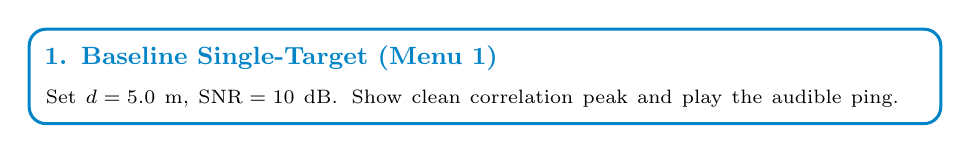
\begin{tikzpicture}
                \node[draw=blueaccent, fill=white, rounded corners=6pt, line width=1.1pt, text width=0.92\linewidth, inner sep=6pt] {
                    \textbf{\textcolor{blueaccent}{\small 1. Baseline Single-Target (Menu 1)}}\\[2pt]
                    \scriptsize Set $d = 5.0\text{ m}$, $\text{SNR} = 10\text{ dB}$. Show clean correlation peak and play the audible ping.
                };
            \end{tikzpicture}
            
            \vspace{4pt}
            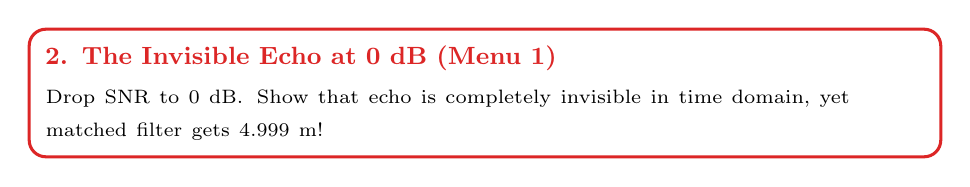
\begin{tikzpicture}
                \node[draw=crimson, fill=white, rounded corners=6pt, line width=1.1pt, text width=0.92\linewidth, inner sep=6pt] {
                    \textbf{\textcolor{crimson}{\small 2. The Invisible Echo at 0 dB (Menu 1)}}\\[2pt]
                    \scriptsize Drop SNR to $0\text{ dB}$. Show that echo is completely invisible in time domain, yet matched filter gets $4.999\text{ m}$!
                };
            \end{tikzpicture}
        \end{column}
        
        \begin{column}{0.48\textwidth}
            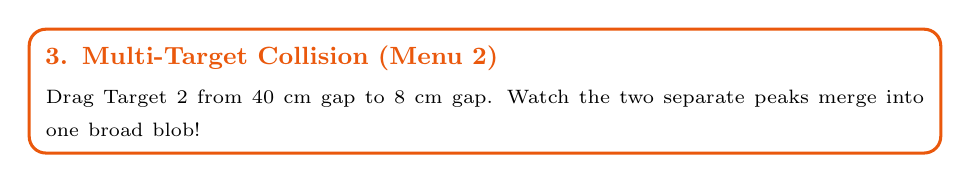
\begin{tikzpicture}
                \node[draw=coral, fill=white, rounded corners=6pt, line width=1.1pt, text width=0.92\linewidth, inner sep=6pt] {
                    \textbf{\textcolor{coral}{\small 3. Multi-Target Collision (Menu 2)}}\\[2pt]
                    \scriptsize Drag Target 2 from $40\text{ cm}$ gap to $8\text{ cm}$ gap. Watch the two separate peaks merge into one broad blob!
                };
            \end{tikzpicture}
            
            \vspace{4pt}
            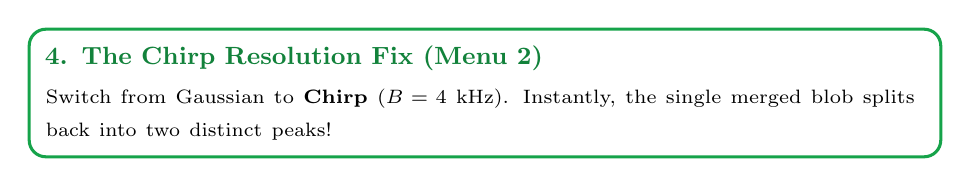
\begin{tikzpicture}
                \node[draw=emerald, fill=white, rounded corners=6pt, line width=1.1pt, text width=0.92\linewidth, inner sep=6pt] {
                    \textbf{\textcolor{emerald!80!black}{\small 4. The Chirp Resolution Fix (Menu 2)}}\\[2pt]
                    \scriptsize Switch from Gaussian to \textbf{Chirp} ($B = 4\text{ kHz}$). Instantly, the single merged blob splits back into two distinct peaks!
                };
            \end{tikzpicture}
        \end{column}
    \end{columns}
    
    \vspace{6pt}
    \centering
    
\begin{tikzpicture}
        \node[draw=navy, fill=navy!5, rounded corners=4pt, inner sep=4pt, text width=0.94\linewidth, align=center] {
            \footnotesize \textbf{Hardware Backup:} Switch to Menu 4 to showcase the physical wall detection at $1.797\text{ m}$ ($6.7\sigma$).
        };
    \end{tikzpicture}
\end{frame}

% ------------------------------------------------------------------------------
% SLIDE 15: TEAM CONTRIBUTIONS
% ------------------------------------------------------------------------------
\begin{frame}{Team Contributions \& Division of Work}{Balanced Collaboration across Signal Processing, Testing, and UI}
    \begin{columns}[T]
        \begin{column}{0.48\textwidth}
            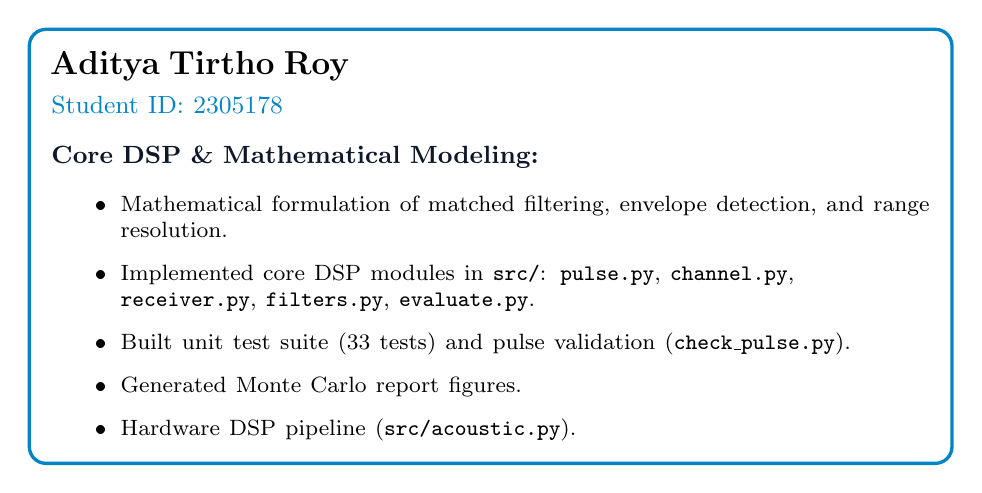
\begin{tikzpicture}
                \node[draw=blueaccent, fill=white, rounded corners=6pt, line width=1.2pt, text width=0.92\linewidth, inner sep=8pt] {
                    \textbf{\large Aditya Tirtho Roy}\\[2pt]
                    \textcolor{blueaccent}{\small Student ID: 2305178}\\[6pt]
                    \textbf{\textcolor{navy}{\small Core DSP \& Mathematical Modeling:}}
                    \begin{itemize}\footnotesize\setlength\itemsep{2pt}
                        \item Mathematical formulation of matched filtering, envelope detection, and range resolution.
                        \item Implemented core DSP modules in \texttt{src/}:
                        \texttt{pulse.py}, \texttt{channel.py}, \texttt{receiver.py}, \texttt{filters.py}, \texttt{evaluate.py}.
                        \item Built unit test suite (33 tests) and pulse validation (\texttt{check\_pulse.py}).
                        \item Generated Monte Carlo report figures.
                        \item Hardware DSP pipeline (\texttt{src/acoustic.py}).
                    \end{itemize}
                };
            \end{tikzpicture}
        \end{column}
        
        \begin{column}{0.48\textwidth}
            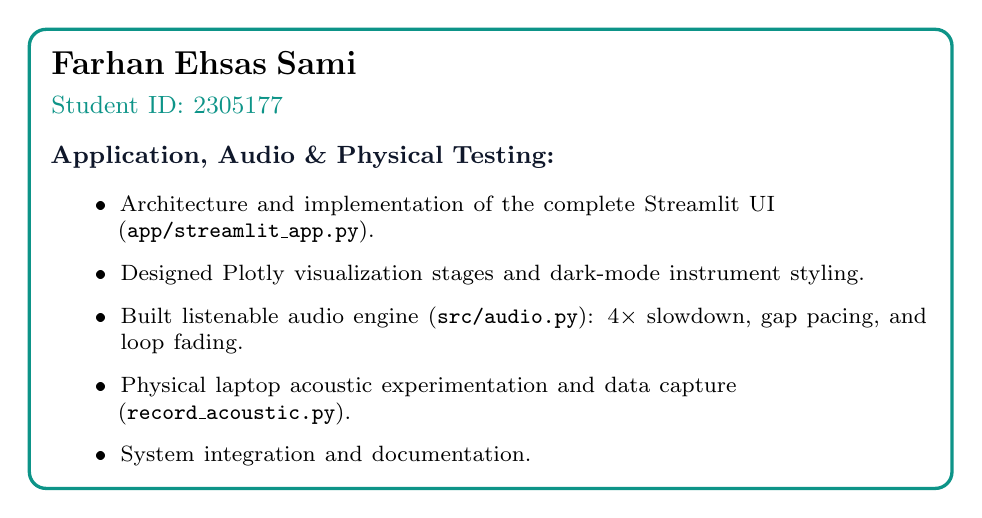
\begin{tikzpicture}
                \node[draw=teal, fill=white, rounded corners=6pt, line width=1.2pt, text width=0.92\linewidth, inner sep=8pt] {
                    \textbf{\large Farhan Ehsas Sami}\\[2pt]
                    \textcolor{teal}{\small Student ID: 2305177}\\[6pt]
                    \textbf{\textcolor{navy}{\small Application, Audio \& Physical Testing:}}
                    \begin{itemize}\footnotesize\setlength\itemsep{2pt}
                        \item Architecture and implementation of the complete Streamlit UI (\texttt{app/streamlit\_app.py}).
                        \item Designed Plotly visualization stages and dark-mode instrument styling.
                        \item Built listenable audio engine (\texttt{src/audio.py}): $4\times$ slowdown, gap pacing, and loop fading.
                        \item Physical laptop acoustic experimentation and data capture (\texttt{record\_acoustic.py}).
                        \item System integration and documentation.
                    \end{itemize}
                };
            \end{tikzpicture}
        \end{column}
    \end{columns}
\end{frame}

% ------------------------------------------------------------------------------
% SLIDE 16: CONCLUSION & KEY TAKEAWAYS
% ------------------------------------------------------------------------------
\begin{frame}{Conclusion: Key Engineering Takeaways}{Connecting Signals \& Systems Theory to Practical Engineering}
    \begin{columns}[T]
        \begin{column}{0.32\textwidth}
            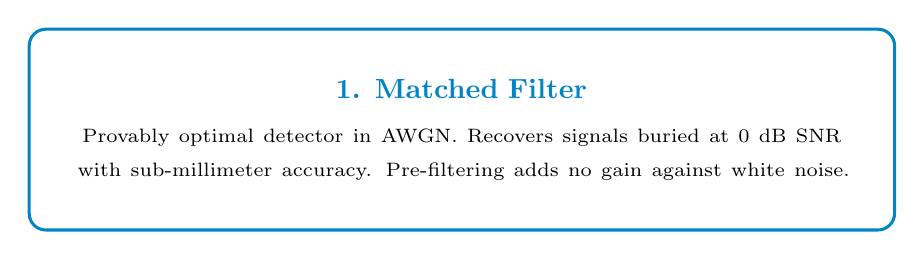
\begin{tikzpicture}
                \node[draw=blueaccent, fill=white, rounded corners=6pt, line width=1.1pt, text width=0.86\linewidth, minimum height=2.55cm, inner sep=8pt, align=center] {
                    \textcolor{blueaccent}{\textbf{\normalsize 1. Matched Filter}}\\[4pt]
                    \scriptsize Provably optimal detector in AWGN. Recovers signals buried at $0\text{ dB}$ SNR with sub-millimeter accuracy. Pre-filtering adds no gain against white noise.
                };
            \end{tikzpicture}
        \end{column}
        
        \begin{column}{0.32\textwidth}
            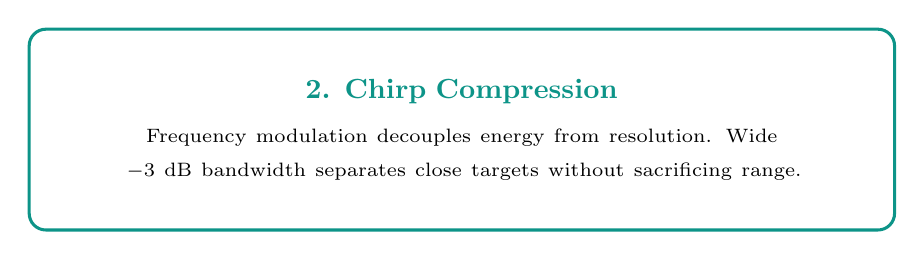
\begin{tikzpicture}
                \node[draw=teal, fill=white, rounded corners=6pt, line width=1.1pt, text width=0.86\linewidth, minimum height=2.55cm, inner sep=8pt, align=center] {
                    \textcolor{teal}{\textbf{\normalsize 2. Chirp Compression}}\\[4pt]
                    \scriptsize Frequency modulation decouples energy from resolution. Wide $-3\text{ dB}$ bandwidth separates close targets without sacrificing range.
                };
            \end{tikzpicture}
        \end{column}
        
        \begin{column}{0.32\textwidth}
            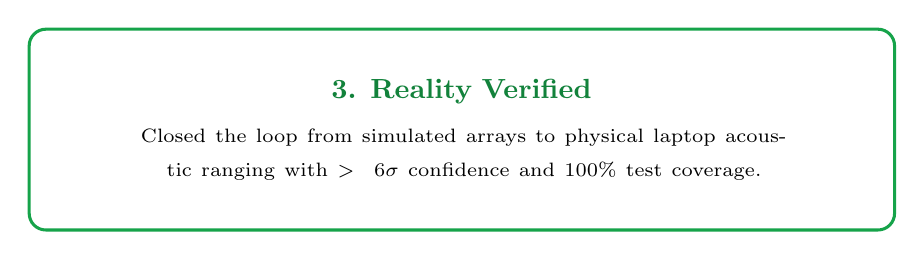
\begin{tikzpicture}
                \node[draw=emerald, fill=white, rounded corners=6pt, line width=1.1pt, text width=0.86\linewidth, minimum height=2.55cm, inner sep=8pt, align=center] {
                    \textcolor{emerald!80!black}{\textbf{\normalsize 3. Reality Verified}}\\[4pt]
                    \scriptsize Closed the loop from simulated arrays to physical laptop acoustic ranging with $>6\sigma$ confidence and 100\% test coverage.
                };
            \end{tikzpicture}
        \end{column}
    \end{columns}
    
    \vspace{16pt}
    \centering
    {\textcolor{navy}{\textbf{\LARGE Thank You!}}}\\[4pt]
    \textcolor{slate}{\small Questions and Discussion Welcomed}
\end{frame}

% ------------------------------------------------------------------------------
% SLIDE 17: ANTICIPATED Q&A DEFENSE
% ------------------------------------------------------------------------------
\begin{frame}{Anticipated Q\&A Defense}{Concise Answers to Critical Examiner Questions}
    \begin{columns}[T]
        \begin{column}{0.5\textwidth}
            \textbf{\textcolor{navy}{\small Q1: Why does RMSE plateau at $\approx 1.8\text{ mm}$ instead of 0?}}
            \begin{itemize}\scriptsize
                \item \textbf{Answer:} Time delay is quantized into integer samples: $k = \text{round}(2d f_s / c)$. Maximum rounding error is $\pm 0.5$ samples. At $f_s = 48\text{ kHz}$, half a sample is:
                $$\Delta d_{\text{quant}} = \frac{c}{4 f_s} = \frac{343}{4 \times 48000} \approx 1.79\text{ mm}$$
            \end{itemize}
            
            \vspace{4pt}
            \textbf{\textcolor{navy}{\small Q2: Why did Butterworth bandpass pre-filter fail to improve RMSE?}}
            \begin{itemize}\scriptsize
                \item \textbf{Answer:} The matched filter transfer function $H(f) = X^*(f)$ already weights each frequency by its signal amplitude. By Cauchy-Schwarz, it is mathematically optimal for AWGN. Pre-filtering out-of-band noise is redundant, while filtering in-band risks attenuating signal power.
            \end{itemize}
        \end{column}
        
        \begin{column}{0.5\textwidth}
            \textbf{\textcolor{navy}{\small Q3: Why raw argmax for single target, but Hilbert for multi-target?}}
            \begin{itemize}\scriptsize
                \item \textbf{Answer:} Single-target ranging achieves highest precision with the sharpest peak (raw correlation argmax). But for multi-targets, raw cross-correlation oscillates at the $4\text{ kHz}$ carrier, creating 15+ false cycle crests. The Hilbert envelope $|\tilde{r}[n]|$ eliminates carrier ripple to reliably count true targets.
            \end{itemize}
            
            \vspace{4pt}
            \textbf{\textcolor{navy}{\small Q4: How did you cancel direct speaker bleed on hardware?}}
            \begin{itemize}\scriptsize
                \item \textbf{Answer:} Speaker-to-mic bleed arrives first ($\approx 10\text{ cm}$) and synchronizes $t=0$. We then coherently fold 16 frames and subtract an empty-room baseline recording (clutter removal), revealing reflections above $6\sigma$.
            \end{itemize}
        \end{column}
    \end{columns}
\end{frame}

\end{document}
